\section{Geodesics and Christoffel Symbols in Extrinsic Geometry}

In these notes we'll cover Geodesics and Christoffel Symbols in extrinsic geometry, so we're going 
to consider 2D surfaces living in a 3D space, and we'll cover the same using intrinsic geometry later.\\

This is also the first step to understanding the concept of Covariant Derivative, but we're getting ahead of ourselves...\\

\textbf{Let's start by defining what a geodesic is, a geodesic is the answer to the question of finding the shortest distance
between two points.}\\

In a flat space, this is pretty easy, the shortest distance between two points is a straight line connecting the two, in mathematical formulation, we 
can write, considering two points defined by vectors $\color{teal}\vec{a}$ and $\color{violet}\vec{b}$:

\begin{equation}
    \begingroup\color{teal}\vec{a}\endgroup + \begingroup\color{brown}\lambda\endgroup(\begingroup\color{violet}\vec{b}\endgroup - \begingroup\color{teal}\vec{a}\endgroup)
\end{equation}

Different values of $\color{brown}\lambda$ gets us any point on the same line.\\

But we generally cannot draw straight lines on a curved 2D surface, so the process of finding the shortest distance 
between two points involves finding a special curve called the \textbf{geodesic}, which is basically the straightest possible path
in a curved surface/space, that also minimizes the distance between two points.\\

To start our discussion on geodesics, we can ask ourselves a pretty basic question: how do we know if a path is straight in a flat space? To answer this, we're 
going to take a look at both velocity and acceleration vectors.

An image talks more than words:

\begin{center}
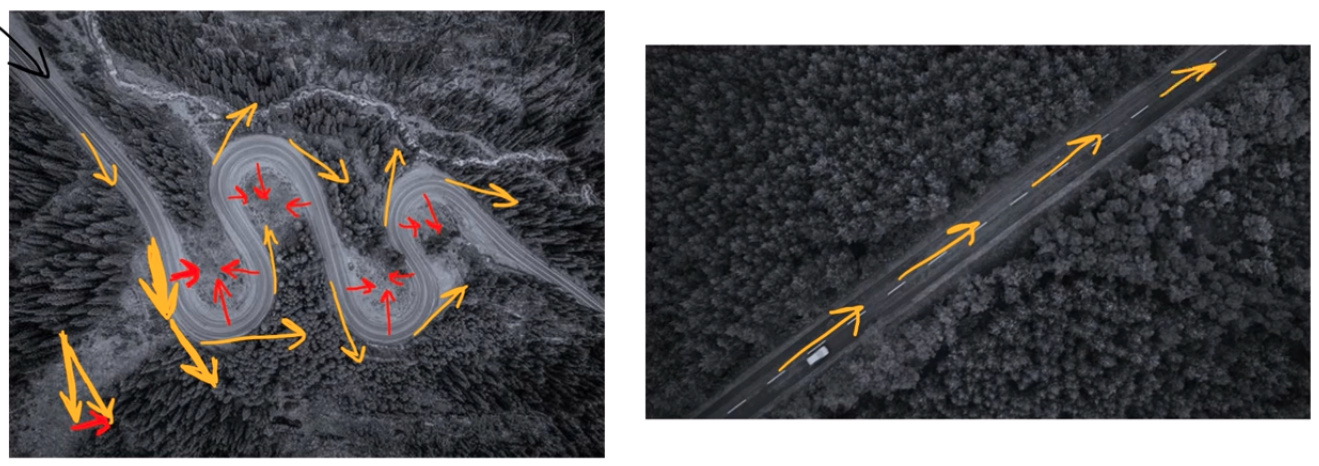
\includegraphics[scale=0.3]{figures/flat-hills.png}
\end{center}

In flat space, a straight path has \textbf{zero acceleration} when we travel along it at constant speed.

\begin{center}
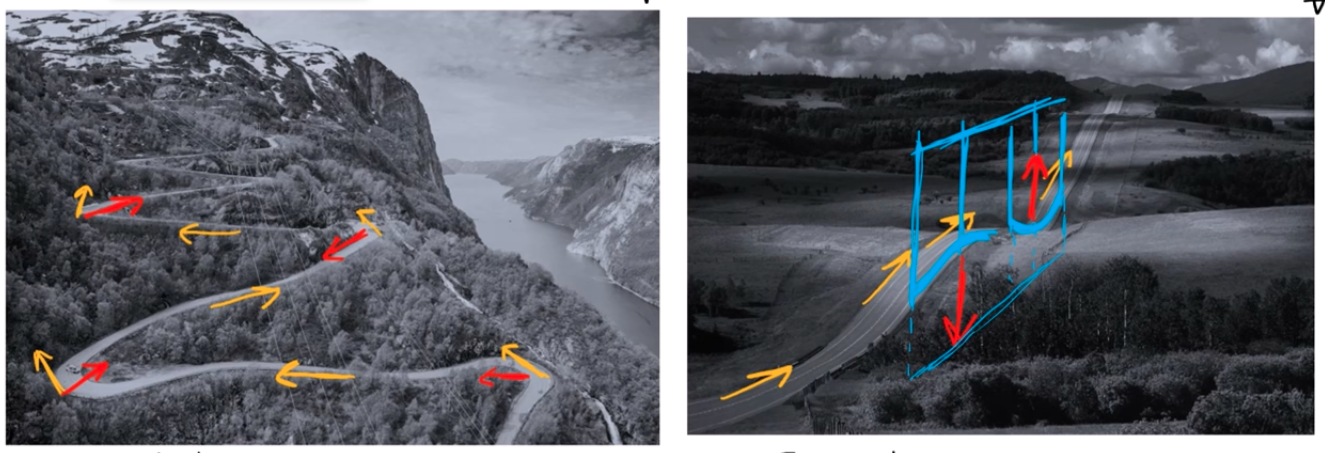
\includegraphics[scale=0.3]{figures/curved-hills.png}
\end{center}

In curved space, a straight path has \textbf{zero tangential acceleration} when we travel along it at constant speed.
The acceleration vector is always pointing out of the surface in the normal direction, for a geodesic curve.\\

And now to the computation of them, we basically need to find curves where the acceleration vector is normal to the surface, so if 
we consider the extrinsic approach, that would mean that, represending the acceleration vector as composed by 
two parts, tangential and normal components, the tangential one would need to be zero:

\begin{align*}
    \frac{d^2 \begingroup\color{violet}\vec{R}\endgroup}{d \begingroup\color{brown}\lambda\endgroup^2} = 
    \cancel{\left(\frac{d^2 \begingroup\color{violet}\vec{R}\endgroup}{d \begingroup\color{brown}\lambda\endgroup^2}\right)^{tangential}} +
    \left(\frac{d^2 \begingroup\color{violet}\vec{R}\endgroup}{d \begingroup\color{brown}\lambda\endgroup^2}\right)^{normal}
\end{align*}

Recall that we've seen how to define a 2D surface using the coordinate system uv and 
the derivatives of the position vector with respect to these u and v coordinates are the tangent basis vectors $\begingroup\color{red}\vec{e_u}\endgroup, \begingroup\color{teal}\vec{e_v}\endgroup$.\\

So to look at the acceleration vector, we need to compute the second order derivative of the position vector with respect to the parameter $\lambda$. We already computed the velocity vector in the 
tangent plane, in \ref{eq:velocity-vector}, using the multi-variable chain-rule:

\begin{equation}
    \frac{d\begingroup\color{violet}\vec{R}\endgroup}{d\begingroup\color{orange}\lambda\endgroup} 
    = \frac{\partial \begingroup\color{violet}\vec{R}\endgroup}{\partial \begingroup\color{red}u\endgroup} \frac{d\begingroup\color{red}u\endgroup}{d\begingroup\color{orange}\lambda\endgroup}
    + \frac{\partial \begingroup\color{violet}\vec{R}\endgroup}{\partial \begingroup\color{teal}v\endgroup} \frac{d\begingroup\color{teal}v\endgroup}{d\begingroup\color{orange}\lambda\endgroup}
\end{equation}

So to get the acceleration vector, we compute the derivative:

\begin{align*}
    \frac{d}{d\begingroup\color{brown}\lambda\endgroup}\left(\frac{d\begingroup\color{violet}\vec{R}\endgroup}{d\begingroup\color{orange}\lambda\endgroup}\right) &=
    \frac{d}{d\begingroup\color{brown}\lambda\endgroup}\left(\frac{\partial \begingroup\color{violet}\vec{R}\endgroup}{\partial \begingroup\color{red}u\endgroup} \frac{d\begingroup\color{red}u\endgroup}{d\begingroup\color{orange}\lambda\endgroup}
    + \frac{\partial \begingroup\color{violet}\vec{R}\endgroup}{\partial \begingroup\color{teal}v\endgroup} \frac{d\begingroup\color{teal}v\endgroup}{d\begingroup\color{orange}\lambda\endgroup}\right)\\
    &= \frac{d}{d\begingroup\color{brown}\lambda\endgroup}\left(\frac{d\begingroup\color{red}u\endgroup}{d\begingroup\color{orange}\lambda\endgroup} \frac{\partial \begingroup\color{violet}\vec{R}\endgroup}{\partial \begingroup\color{red}u\endgroup}\right)
    + \frac{d}{d\begingroup\color{brown}\lambda\endgroup}\left(\frac{d\begingroup\color{teal}v\endgroup}{d\begingroup\color{orange}\lambda\endgroup} \frac{\partial \begingroup\color{violet}\vec{R}\endgroup}{\partial \begingroup\color{teal}v\endgroup}\right)\\
    &= \frac{d^2 \begingroup\color{red}u\endgroup}{d\begingroup\color{brown}\lambda\endgroup^2}\frac{\partial \begingroup\color{violet}\vec{R}\endgroup}{\partial \begingroup\color{red}u\endgroup} 
    + \frac{d \begingroup\color{red}u\endgroup}{d\begingroup\color{brown}\lambda\endgroup} \left(\frac{d}{d\begingroup\color{orange}\lambda\endgroup} \frac{\partial \begingroup\color{violet}\vec{R}\endgroup}{\partial \begingroup\color{red}u\endgroup}\right)
    + \frac{d^2 \begingroup\color{teal}v\endgroup}{d\begingroup\color{brown}\lambda\endgroup^2}\frac{\partial \begingroup\color{violet}\vec{R}\endgroup}{\partial \begingroup\color{teal}v\endgroup} 
    + \frac{d \begingroup\color{teal}v\endgroup}{d\begingroup\color{brown}\lambda\endgroup} \left(\frac{d}{d\begingroup\color{orange}\lambda\endgroup} \frac{\partial \begingroup\color{violet}\vec{R}\endgroup}{\partial \begingroup\color{teal}v\endgroup}\right)
\end{align*}

The terms containing the second order derivatives of $\color{red}u$ and $\color{teal}v$ are okay to understand, but the other two terms, where we see the derivative
of the basis vectors with respect to the parameter $\color{brown}\lambda$ require some additional work to figure out correctly.\\
We know from multi-variable chain rule, that the $\color{brown}\lambda$ derivative operator, can be explanded out as a linear combination of 
$\color{red}u$ and $\color{teal}v$ derivative operators:

\begin{equation}
    \frac{d}{d\begingroup\color{brown}\lambda\endgroup} = \frac{d\begingroup\color{red}u\endgroup}{d\begingroup\color{brown}\lambda\endgroup} \frac{\partial}{\partial \begingroup\color{red}u\endgroup} + 
    \frac{d\begingroup\color{teal}v\endgroup}{d\begingroup\color{brown}\lambda\endgroup} \frac{\partial}{\partial \begingroup\color{teal}v\endgroup}
\end{equation}

So, the two derivatives above can be expressed as:

\begin{align*}
    \frac{d}{d\begingroup\color{brown}\lambda\endgroup} \frac{\partial \begingroup\color{violet}\vec{R}\endgroup}{\partial \begingroup\color{red}u\endgroup} 
    &= \left(\frac{d\begingroup\color{red}u\endgroup}{d\begingroup\color{brown}\lambda\endgroup} \frac{\partial}{\partial \begingroup\color{red}u\endgroup} + 
    \frac{d\begingroup\color{teal}v\endgroup}{d\begingroup\color{brown}\lambda\endgroup} \frac{\partial}{\partial \begingroup\color{teal}v\endgroup}\right)
    \frac{\partial \begingroup\color{violet}\vec{R}\endgroup}{\partial \begingroup\color{red}u\endgroup}\\
    &= \frac{d\begingroup\color{red}u\endgroup}{d\begingroup\color{brown}\lambda\endgroup} \frac{\partial^2 \begingroup\color{violet}\vec{R}\endgroup}{\partial \begingroup\color{red}u\endgroup^2}
    + \frac{d\begingroup\color{teal}v\endgroup}{d\begingroup\color{brown}\lambda\endgroup} \frac{\partial^2 \begingroup\color{violet}\vec{R}\endgroup}{\partial \begingroup\color{red}u\endgroup \partial\begingroup\color{teal}v\endgroup}\\\\
    \frac{d}{d\begingroup\color{brown}\lambda\endgroup} \frac{\partial \begingroup\color{violet}\vec{R}\endgroup}{\partial \begingroup\color{teal}v\endgroup} 
    &= \left(\frac{d\begingroup\color{red}u\endgroup}{d\begingroup\color{brown}\lambda\endgroup} \frac{\partial}{\partial \begingroup\color{red}u\endgroup} + 
    \frac{d\begingroup\color{teal}v\endgroup}{d\begingroup\color{brown}\lambda\endgroup} \frac{\partial}{\partial \begingroup\color{teal}v\endgroup}\right)
    \frac{\partial \begingroup\color{violet}\vec{R}\endgroup}{\partial \begingroup\color{teal}v\endgroup}\\
    &= \frac{d\begingroup\color{red}u\endgroup}{d\begingroup\color{brown}\lambda\endgroup} \frac{\partial^2 \begingroup\color{violet}\vec{R}\endgroup}{\partial \begingroup\color{teal}v\endgroup \partial\begingroup\color{red}u\endgroup}
    + \frac{d\begingroup\color{teal}v\endgroup}{d\begingroup\color{brown}\lambda\endgroup} \frac{\partial^2 \begingroup\color{violet}\vec{R}\endgroup}{\partial\begingroup\color{teal}v\endgroup^2}
\end{align*}

So we can now substitute in the previous expression of the acceleration vector:

\begin{align*}
    \frac{d}{d\begingroup\color{brown}\lambda\endgroup}\left(\frac{d\begingroup\color{violet}\vec{R}\endgroup}{d\begingroup\color{orange}\lambda\endgroup}\right) &= 
    \frac{d^2 \begingroup\color{red}u\endgroup}{d\begingroup\color{brown}\lambda\endgroup^2}\frac{\partial \begingroup\color{violet}\vec{R}\endgroup}{\partial \begingroup\color{red}u\endgroup} 
    + \frac{d \begingroup\color{red}u\endgroup}{d\begingroup\color{brown}\lambda\endgroup} \left(\frac{d}{d\begingroup\color{orange}\lambda\endgroup} \frac{\partial \begingroup\color{violet}\vec{R}\endgroup}{\partial \begingroup\color{red}u\endgroup}\right)
    + \frac{d^2 \begingroup\color{teal}v\endgroup}{d\begingroup\color{brown}\lambda\endgroup^2}\frac{\partial \begingroup\color{violet}\vec{R}\endgroup}{\partial \begingroup\color{teal}v\endgroup} 
    + \frac{d \begingroup\color{teal}v\endgroup}{d\begingroup\color{brown}\lambda\endgroup} \left(\frac{d}{d\begingroup\color{orange}\lambda\endgroup} \frac{\partial \begingroup\color{violet}\vec{R}\endgroup}{\partial \begingroup\color{teal}v\endgroup}\right)\\
    &=
\end{align*}

